%%%%----------------------------------------------------------------------------------------
\begin{frame}
\frametitle{Appendix:}
\framesubtitle{Aleatoric to epistemic}
\begin{figure}[!ht]       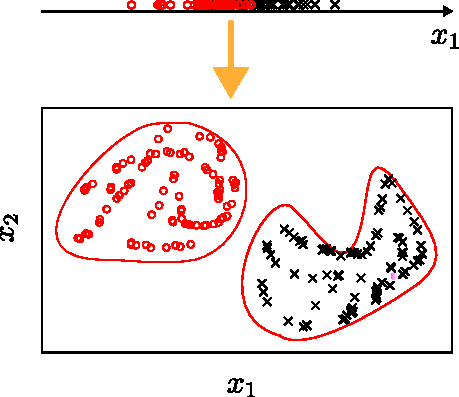
\includegraphics[scale=1]{figures/figure-transform.pdf}
\end{figure}
    
\end{frame}
%%%%----------------------------------------------------------------------------------------
\begin{frame}
\frametitle{Appendix:}
\framesubtitle{Sequential Bayesian inference}
\begin{figure}[!ht]       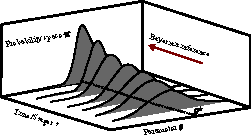
\includegraphics[scale=2.55]{figures/figure-SBI.pdf}
\end{figure}
    
\end{frame}


%=====================================================

%================================================
\begin{frame}
\frametitle{Appendix:}
\framesubtitle{Inverse probability transform}
\begin{itemize}
    \item Inverse probability transform
\end{itemize}
\begin{figure}[ht]
    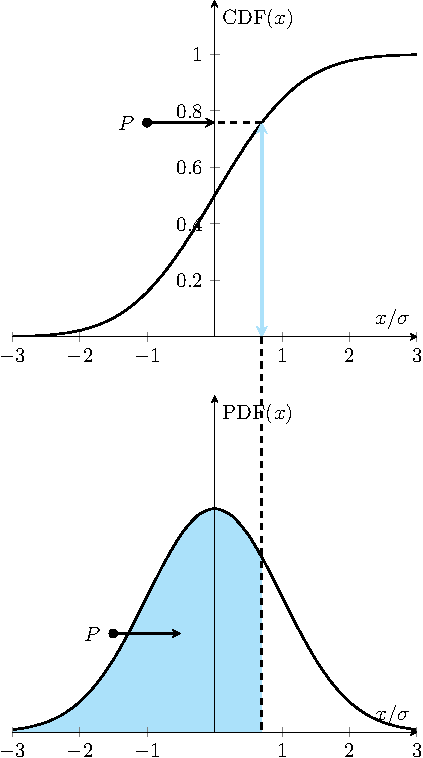
\includegraphics[width = 35mm]{figures/figure-CDF.pdf}
\end{figure}
\end{frame}
%================================================

\begin{frame}
\frametitle{Appendix:}
\framesubtitle{Rejection sampling}
\begin{itemize}
    \item Rejection sampling
\end{itemize}
\begin{figure}[ht]
    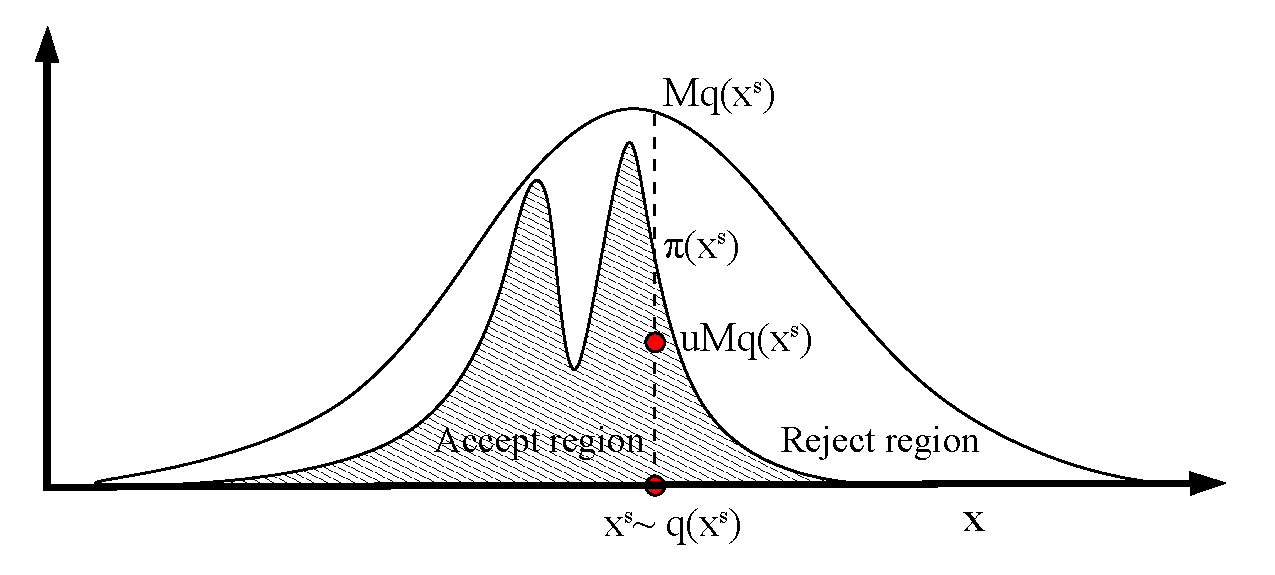
\includegraphics[width = 110mm]{figures/figure-rejectionsampling.pdf}
\end{figure}
\end{frame}
%================================================

\begin{frame}
\frametitle{Appendix:}
\framesubtitle{importance sampling}
\begin{equation*}
E[f(\boldsymbol{x}_{t})] = \int f(\boldsymbol{x}_{t})\pi(\boldsymbol{x}_{t}) d\boldsymbol{x}_{t}
\approx \frac{1}{S}\sum_{s=1}^{S} f(\boldsymbol{x}_{t}^{s})
\end{equation*}


\begin{equation*}
    E[f(\boldsymbol{x}_{t})] = \int f(\boldsymbol{x}_{t})\pi(\boldsymbol{x}_{t}) d\boldsymbol{x}_{t} = \int f(\boldsymbol{x}_{t})\frac{\pi(\boldsymbol{x}_{t})}{q(\boldsymbol{x}_{t})}q(\boldsymbol{x}_{t}) d\boldsymbol{x}_{t}
    \approx \frac{1}{S} \sum_{s=1}^{S} f(\boldsymbol{x}_{t}^{s})\frac{\pi(\boldsymbol{x}_{t}^{s})}{q(\boldsymbol{x}_{t}^{s})}
\end{equation*}

    \begin{itemize}
        \item Require a proper proposal distribution $q(\boldsymbol{x}_{t})$

    \end{itemize}

\end{frame}
%=======================================================
\begin{frame}
\frametitle{Appendix:}
\framesubtitle{Metropolish-Hasting}
\begin{equation*}
f(\boldsymbol{x}_{t}^{s+1}|\boldsymbol{x}_{t}^{s})=\rm{min}(1,\alpha)
\end{equation*}
\begin{equation*}
\alpha = {\rm{min}} (1,
\frac{q(\boldsymbol{x}_{t}^{s}|\boldsymbol{x}_{t}^{s+1})  \pi(\boldsymbol{x}_{t}^{s+1}|\mathcal{Y}_{t})}
{q(\boldsymbol{x}_{t}^{s+1}|\boldsymbol{x}_{t}^{s})   \pi(\boldsymbol{x}_{t}^{s}|\mathcal{Y}_{t})} )
\end{equation*}

\end{frame}
%============================================================
\begin{frame}
\frametitle{Appendix:}
\framesubtitle{Metropolish-Hasting}
\begin{algorithm}[H]
    \caption{MH algorithm at $t_{th}$ step}
    \label{Algorithm:MH}
    \KwData{ $q(\boldsymbol{x}_{t})$: Proposal distribution; $\pi(\boldsymbol{x}_{t}|\mathcal{Y})$: Target posterior.}
    \KwResult{MCMC samples at $t_{th}$ stage: $\mathcal{X}_{t} = \{\boldsymbol{x}_{t}^{1},\cdots,\boldsymbol{x}_{t}^{N_{\mathcal{X}}}\}$}
    Initialization $\boldsymbol{x}_{t}^{1} \in \mathcal{D}_{\bm{X}}$\; 
    \For{$s \gets 2 \ to  \ N_{\mathcal{X}}$}{
        Sample $\boldsymbol{x}_{t}^{s+1} \sim q(\boldsymbol{x}_{t}^{s+1}|\boldsymbol{x}_{t}^{s})$;\\
        Compute acceptance probability $\alpha$;\\
        Compute $f\left(\boldsymbol{x}_{t}^{s+1}|\boldsymbol{x}_{t}^s\right)=\min{\left(1,\alpha\right)}$;\\
        Sample $u \sim \mathcal{U}\left(0,1\right)$;\\
        Set candidate sample $\boldsymbol{x}_{t}^{(\star)}$ to $\boldsymbol{x}_{t}^{s+1}$ with probability $\alpha$;} 
\end{algorithm}
\end{frame}
%======================================================================================
\begin{frame}
\frametitle{Appendix:}
\framesubtitle{Metropolish-Hasting}
\begin{figure}[ht]
    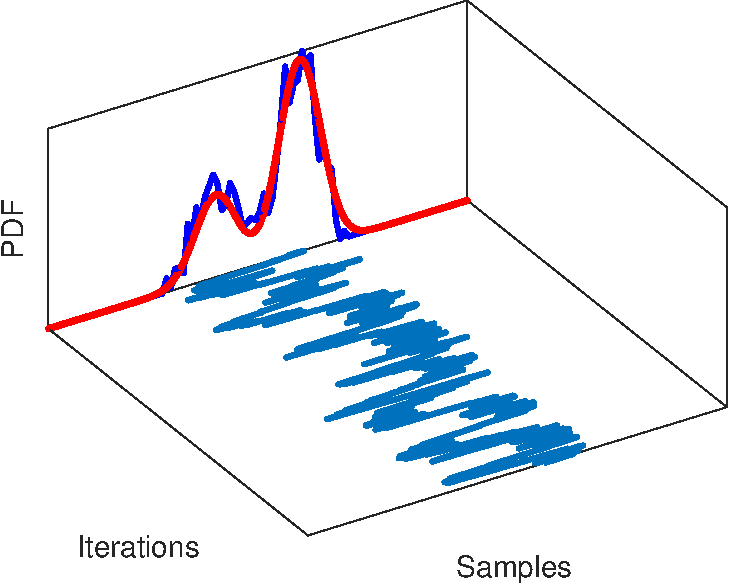
\includegraphics[width = 80mm]{figures/figure-MCMC_sampling.pdf}
\end{figure}
\end{frame}


%=============================================================================
\begin{frame}
\frametitle{Appendix:}
\framesubtitle{AIES}
\begin{equation*}
\boldsymbol{x}_{t}^{(\star)}
=
\boldsymbol{x}_{t\_i}^{(s)}
+
z \cdot 
(\boldsymbol{x}_{t\_j}^{(\tilde{s})} - \boldsymbol{x}_{t\_i}^{(s)})
\end{equation*}
\begin{equation*}
    p(z|a)= \left\{\begin{matrix}
  \frac{1}{\sqrt{z} (2\sqrt{a} - \frac{2}{\sqrt{a} } )}  & {\rm{if} }\ z \in [1 / a, a]  \\
  0 & {\rm{otherwise} }
\end{matrix}\right.
\end{equation*}
\begin{equation*}
    \alpha = {\rm{min}}
(1,
z^{M-1} 
\frac{\pi({x}_{t}^{(\star)}|\mathcal{Y})}
{\pi({x}_{t\_{i}}^{(s)}|\mathcal{Y})} 
)
\end{equation*}
\end{frame}

%=========================================================
\begin{frame}
\frametitle{Appendix:}
\framesubtitle{AIES}
\begin{algorithm}[H]    
    \caption{AIES algorithm at $t_{th}$ step}
    \label{Algorithm:AIES}
    \KwData{$\pi(\boldsymbol{x}_{t}|\mathcal{Y})$: Target posterior; tuning parameter $a$}
    \KwResult{MCMC samples at $t_{th}$ stage: $\mathcal{X}_{t} = \{ \mathcal{X}_{t\_1},\cdots,\mathcal{X}_{t\_N_{chain}}\}$), with $\mathcal{X}_{t\_i}=\{ \boldsymbol{x}_{t\_i}^{1},\cdots,\boldsymbol{x}_{t\_i}^{N_{\mathcal{X}}}\}$}
    Initialization $N_{chain}$ samples $\{  \boldsymbol{x}_{t\_1}^{1},\cdots,\boldsymbol{x}_{t\_{N_{chain}}}^{1}\}$, with $\boldsymbol{x}_{t\_i}^{1} \in \mathcal{D}_{\boldsymbol{X}}$\
    
    \For{$s \gets 2 \ to  \ N_{\mathcal{X}}$}{
        \For{$ i \in \{ 1,\cdots,N_{chain}\}$}{
            Pick random $j$ from $\{ 1,\cdots,N_{chain}\} \backslash i$;\\
            Propose ${x}_{t}^{(\star)}$ with \cref{eq: AIES walker};\\
            Set $\boldsymbol{x}_{t\_i}^{s} = {x}_{t}^{(\star)}$ with probability $\alpha$ (see \cref{eq: AIES acceptance probability});
        }        
        } 
\end{algorithm}
\end{frame}
%=====================================================================================
\begin{frame}
\frametitle{Appendix:}
\framesubtitle{Sequential Monte Carlo}
\begin{equation*}
\label{eq: Bayesian filtering}
\begin{aligned}
   & \boldsymbol{{x}_{t}}  =g(\boldsymbol{{x}_{t-1}}) + \boldsymbol{v} \ \   \ &\rm{(state  \ equation)}\\    
     &\mathcal{Y}_{t}=m(\boldsymbol{{x}_{t}}) + \boldsymbol{w} \ \ \ \ \ &\rm{(observation \  equation)}
\end{aligned}
\end{equation*}

\begin{equation*}
\pi(\boldsymbol{x}_{1:t}|\mathcal{Y}_{1:t})
\approx 
\sum_{s=1}^{S} 
\tilde{w}_{t}^{s}
\delta_{\boldsymbol{x}_{1:t}^{s}}(\boldsymbol{x}_{1:t})
\end{equation*}

\begin{equation*}
\tilde{w}_t^s=\frac{w_t^s}{\sum_{s=1}^{S}{(w_t^s)}}
\end{equation*}

\begin{equation*}
\pi(\boldsymbol{x}_{1:t}|\mathcal{Y}_{1:t})
    \propto 
    \pi(\mathcal{Y}_{t}|\boldsymbol{x}_{t})
    \pi(\boldsymbol{x}_{t}|\boldsymbol{x}_{t-1})
    \pi(\boldsymbol{x}_{t-1}|\mathcal{Y}_{t-1})
\end{equation*}
\end{frame}

%======================================================
\begin{frame}
\frametitle{Appendix:}
\framesubtitle{Sequential Monte Carlo}
\begin{figure}[ht]
    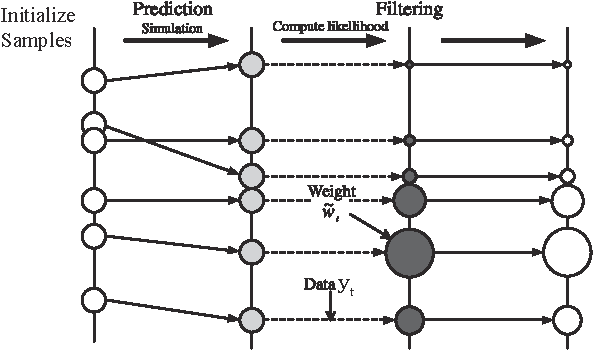
\includegraphics[width = 110mm]{figures/figure-PF-SIS.pdf}
\end{figure}
\end{frame}
%===================================================
\begin{frame}
\frametitle{Appendix:}
\framesubtitle{Sequential Monte Carlo with resampling}
\begin{algorithm}[H]    
    \caption{SISR algorithm at $t_{th}$ step}
    \label{Algorithm:SISR}
    \KwData{Samples $\boldsymbol{x}_{t-1}^{s}$ with weights $w_{t-1}^{s},\ s = \{1,\cdots,N\}$; observation $\mathcal{Y}_{t}$ at $t_{th}$ stage}
    \KwResult{SMC samples with normalized weights $\tilde{w}_{t}^{s}$ at $t_{th}$ stage: $\boldsymbol{x}_{t}^{(\star)} = \{\boldsymbol{x}_{t}^{1},\cdots,\boldsymbol{x}_{t}^{N} \}$)}
    \For{$s \gets 1 \ to  \ N$}{
            Sample from proposal distribution $\boldsymbol{x}_{t}^{s} \sim q(\boldsymbol{x}_{t}^{s}|\boldsymbol{x}_{t-1}^{s},\mathcal{Y}_{t})$;\\
            Compute weight using \cref{eq: PF-modified_weight};
        } 
        Normalized weights;\\
        Calculate degeneracy measure using \cref{eq: SISR_Seff};\\
        \If{$\hat{S}_{eff} < S$}{
        Resample;\\        
        }
\end{algorithm}
\end{frame}
%=====================================================================
\begin{frame}
\frametitle{Appendix:}
\framesubtitle{Sequential Monte Carlo with resampling}
\begin{figure}[ht]
    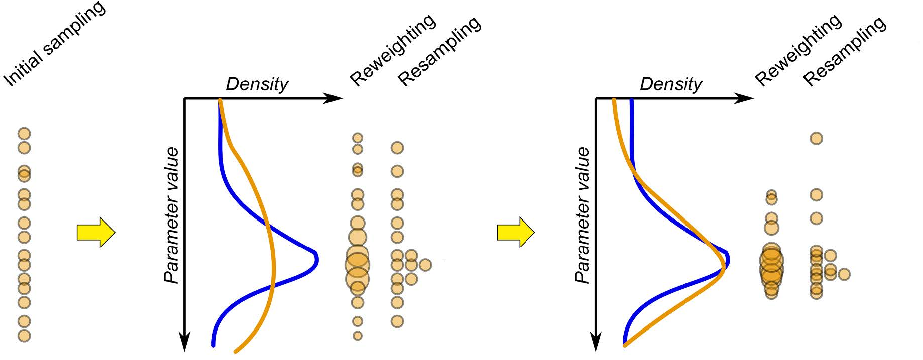
\includegraphics[width = 130mm]{figures/figure-PF-SISR.pdf}
\end{figure}
\end{frame}

%======================================================
\begin{frame}
\frametitle{Appendix:}
\framesubtitle{Visualized PCE}
\begin{figure}[ht]
    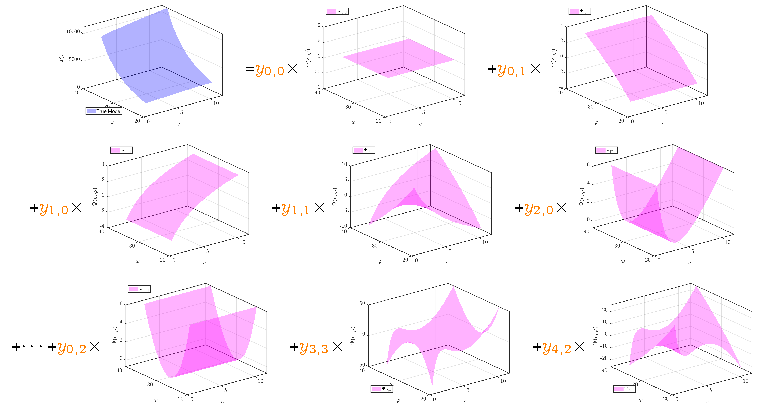
\includegraphics[width = 130mm]{figures/figure-PCE_visualize.pdf}
\end{figure}
\end{frame}